\section{Architektur}
    \label{section:Architecture}
    Das \gls{wccs} verwendet eine Microservices-Architektur.
    Dieses Muster wird in diesem Kapitel zuerst vorgestellt.
    Anschließend erläutert es die konkrete Architektur des Systems.

    \subsection{Microservices Architekturen}
        \paragraph{Prinzipien}
        \paragraph{Vorteile}
        \paragraph{Herausforderungen}

    \subsection{Architektur}
        % TODO Sollte WCCS component lieber WCCS service sein? Was mit DSL oder Crawler? Was wären das dann?
        Architektur wird in zwei Schritten vorgestellt.
        Zunächst ein Blick in den internen Aufbau und anschließend auf die Zusammenhänge mit der Außenwelt.
        
        Abbildung \ref{image:wccsInternalArchitecture} legt den Fokus auf die
        internen Abläufe und Komponenten.

        \begin{figure}
            \centering
            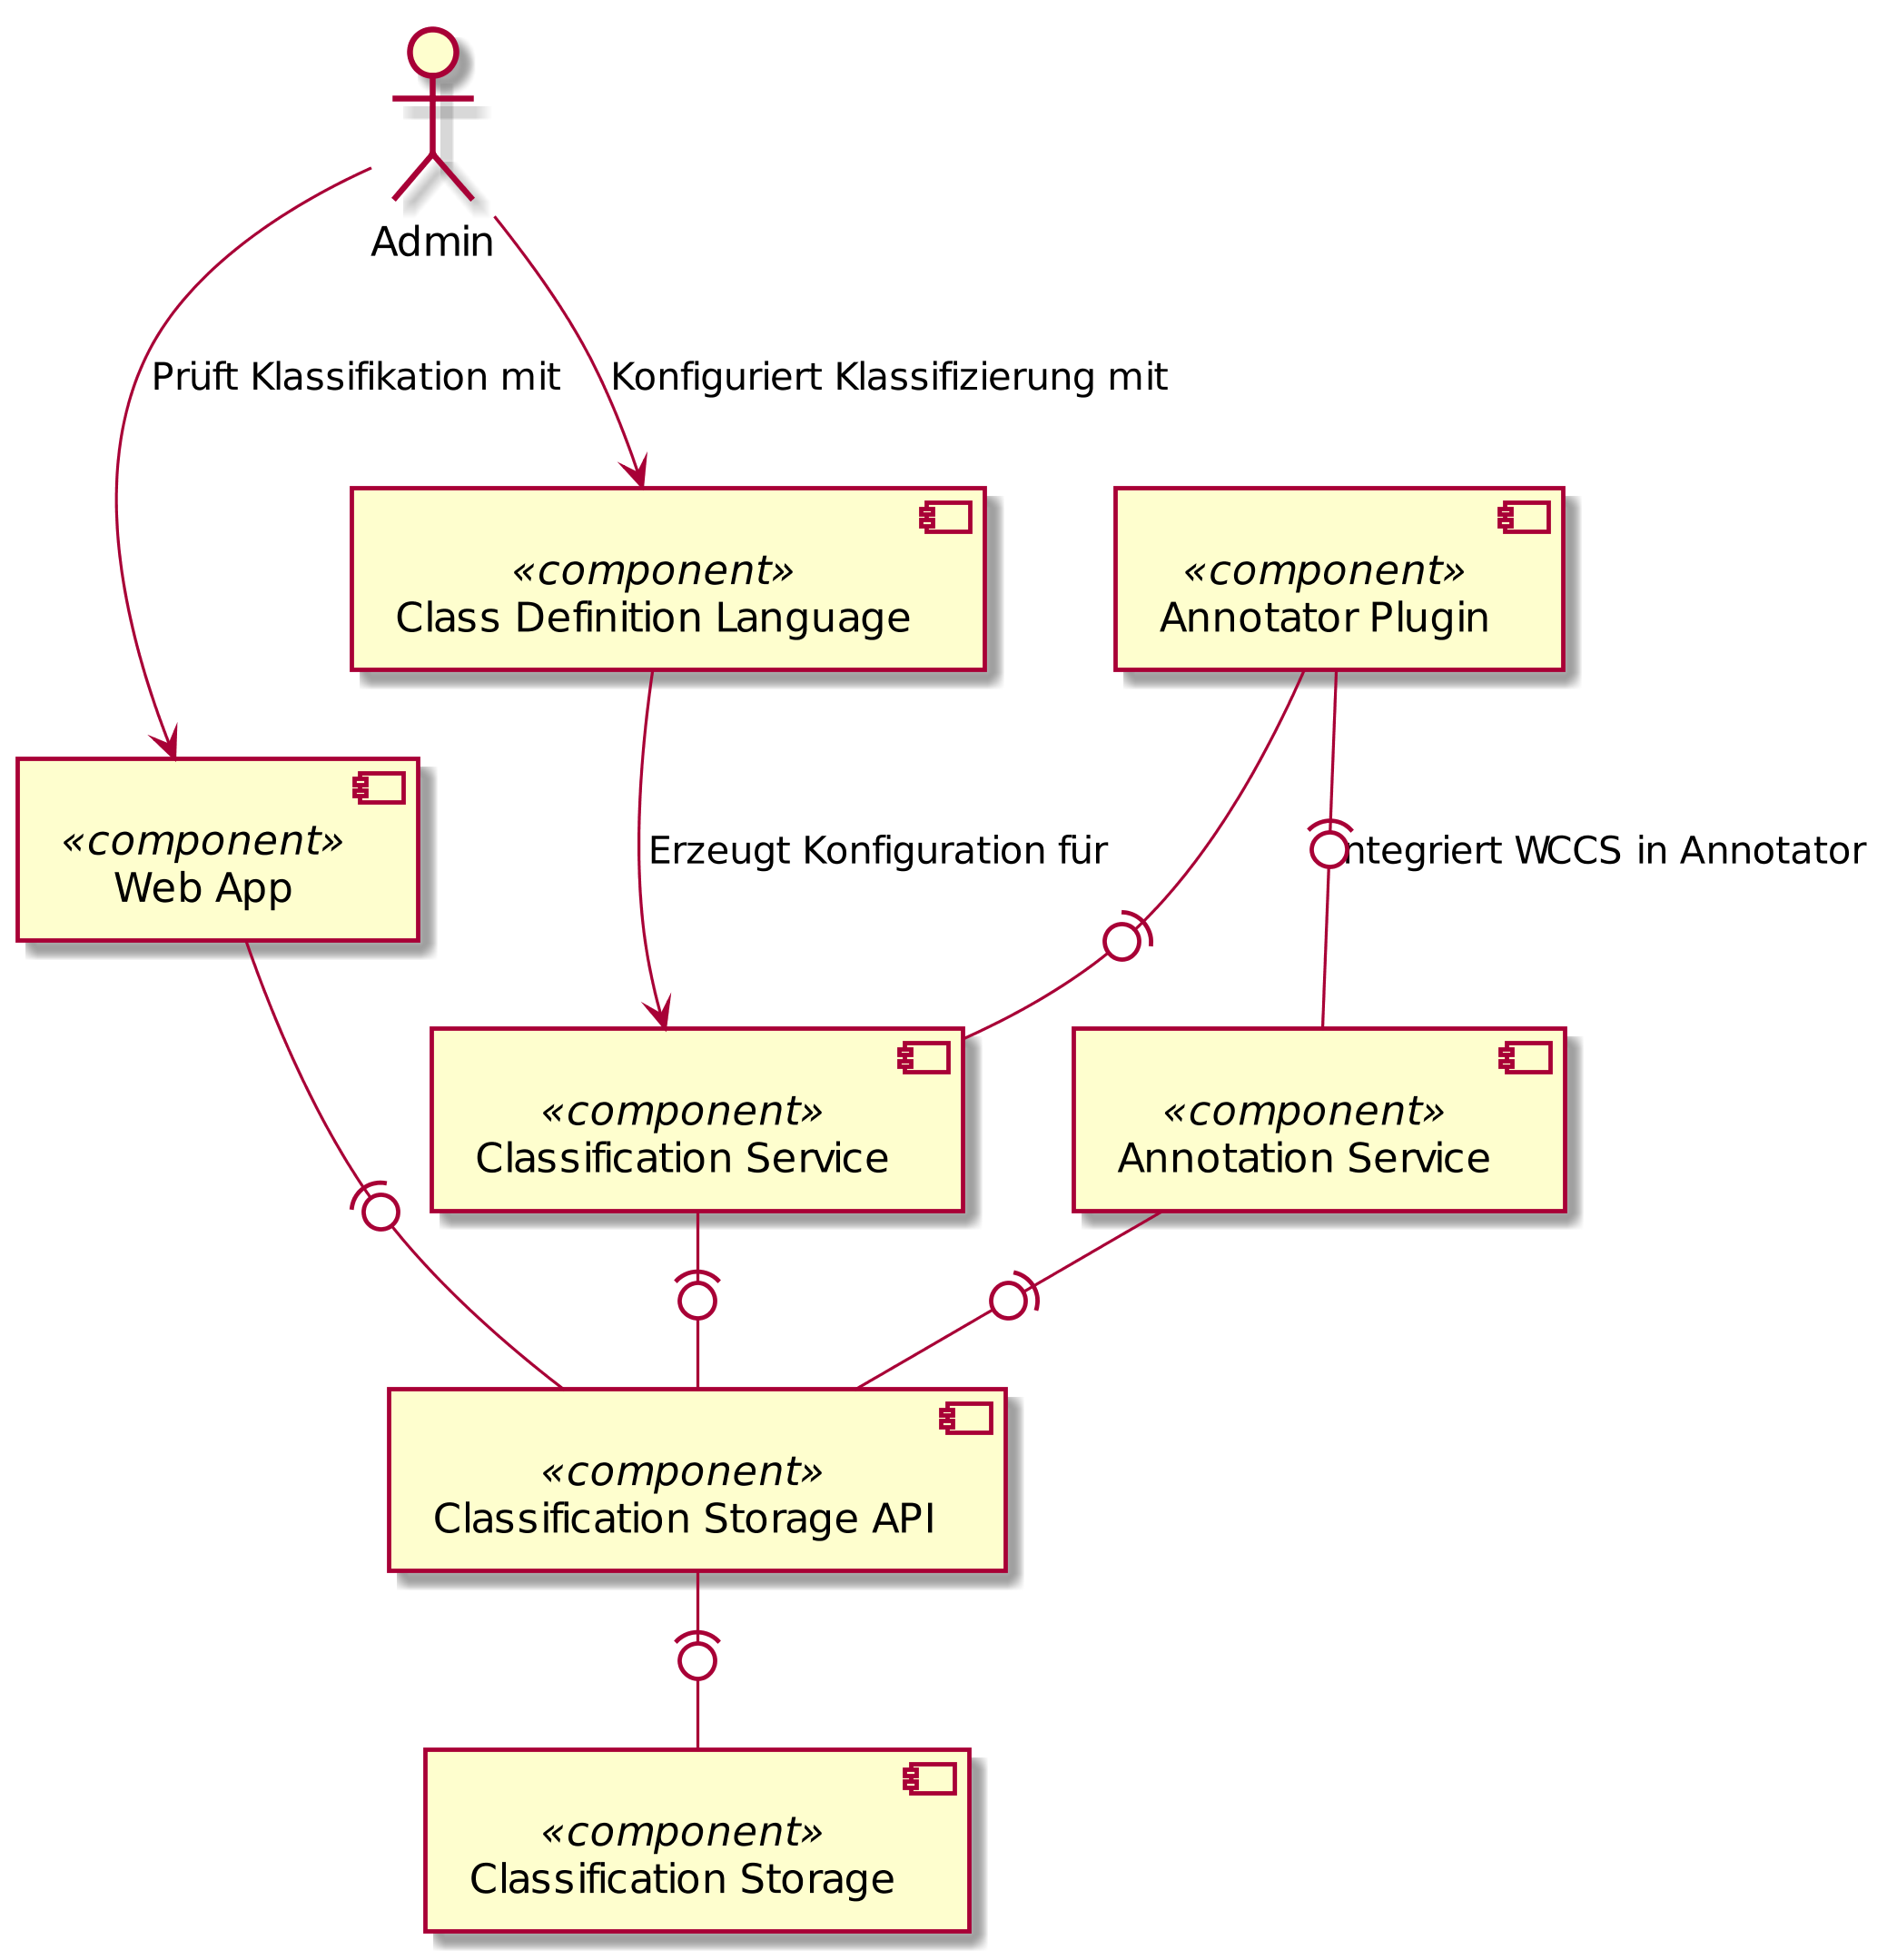
\includegraphics[width=0.7\textwidth]{../resources/architecture/wccs_internal_architecture.png}
            \caption{Interne Architkektur von WCCS}
            \label{image:wccsInternalArchitecture}
        \end{figure}

        Das \gls{wccs} besteht aus fünf Services im Sinne einer Micro-Services-Architektur.
        Dem Classification Storage, der Classification Storage API, dem Classification Service, dem
        Annotation Service und der Web App.

        Der Service Classification Storage stellt die Persistenz bereit und speichert
        Klassifikationen in einer Datenbank.
        Seine Schnittstelle entspricht der der verwendeten Datenbank und ist deshalb
        technisch orientiert.
        Mehr dazu in Kapitel \ref{section:solutionDetailsPersistence}.

        Die Classification Storage bietet eine fachliche Schnittstelle für die Datenhaltung.
        Er übersetzt deshalb fachliche Anfragen in Anfragen in der Sprache der Datenbank.
        Dementsprechend ist die konkrete Implementierung dieses Services abhängig vom Classification Storage.
        Die Schnittstelle der API - eine REST-Schnittstell - ist allerdings fachlich und deshalb
        unabhängig. Mehr zu diesem Service steht in  Kapitel \ref{section:solutionDetailsStorageAPI}.

        Der Classification Service führt die eigentliche Klassifizierung durch
        und speichert das Ergebnis über die Classification Storage API.
        Der Service kann ebenfalls über eine REST-Schnittstelle angesprochen werden.
        Mehr zum Service steht in Kapitel \ref{section:solutionDetailsClassificationService}.

        Der Annotation Service transformiert eine Klassifikation,
        die er über den Classification Storage bezieht,
        in eine Menge von Annotationen.
        Neben der Abfrage von Annotationen bietet seine Schnittstelle auch
        die Möglichkeit solche zu aktualisieren.
        Das technische Format orientiert sich an dem der Annotation Library.
        Mehr steht in Kapitel \ref{section:solutionDetailsAnnotationService}.

        Der verbliebene Service - die Web App - ist im Kern ein Web-Server,
        der die Web Anwendung bereitstellt,
        mit der der Nutzer die Klassifikation prüfen kann.
        Diese bezieht die Anwendung über die Classification Storage API ab.

        Neben diesen Services besitzt das System weitere Komponenten:
        Die Web Content Class Definition Language und das Plugin für die
        Annotation Library.
        Die Sprache nutzt der Admin, um eine Konfigurationsdatei für den
        Classification Service zu erstellen.
        Mehr zur Sprache in Kapitel \ref{section:solutionDetailsDSL}.
        Das Annotator Plugin stellt eine Integration des \gls{wccs} in
        Annotator dar.
        Es bezieht die Annotationen einer Seite über den Annotation Service
        und Informationen über bekannte Klassen vom Classification Service.
        Beides ist notwendig, um einem Anwender die Klassifikation zu visualisieren
        und modifizierbar zu machen.
        Details in Kapitel \ref{section:solutionDetailsAnnotatorPlugin}.

        Die bisherige Betrachtung beantwortet noch nicht die Fragen,
        von wem der Classification Service angesprochen wird und wer das Annotator Plugin einbindet.
        Genauso ist noch offen, welche weiteren Beziehungen zur Umgebung bestehen.

        Das stellt Abbildung \ref{image:wccsExternalArchitecture} dar
        und enthält neben einigen Komponenten des \gls{wccs} vor allem auch
        externe Komponenten.

        \begin{figure}
            \centering
            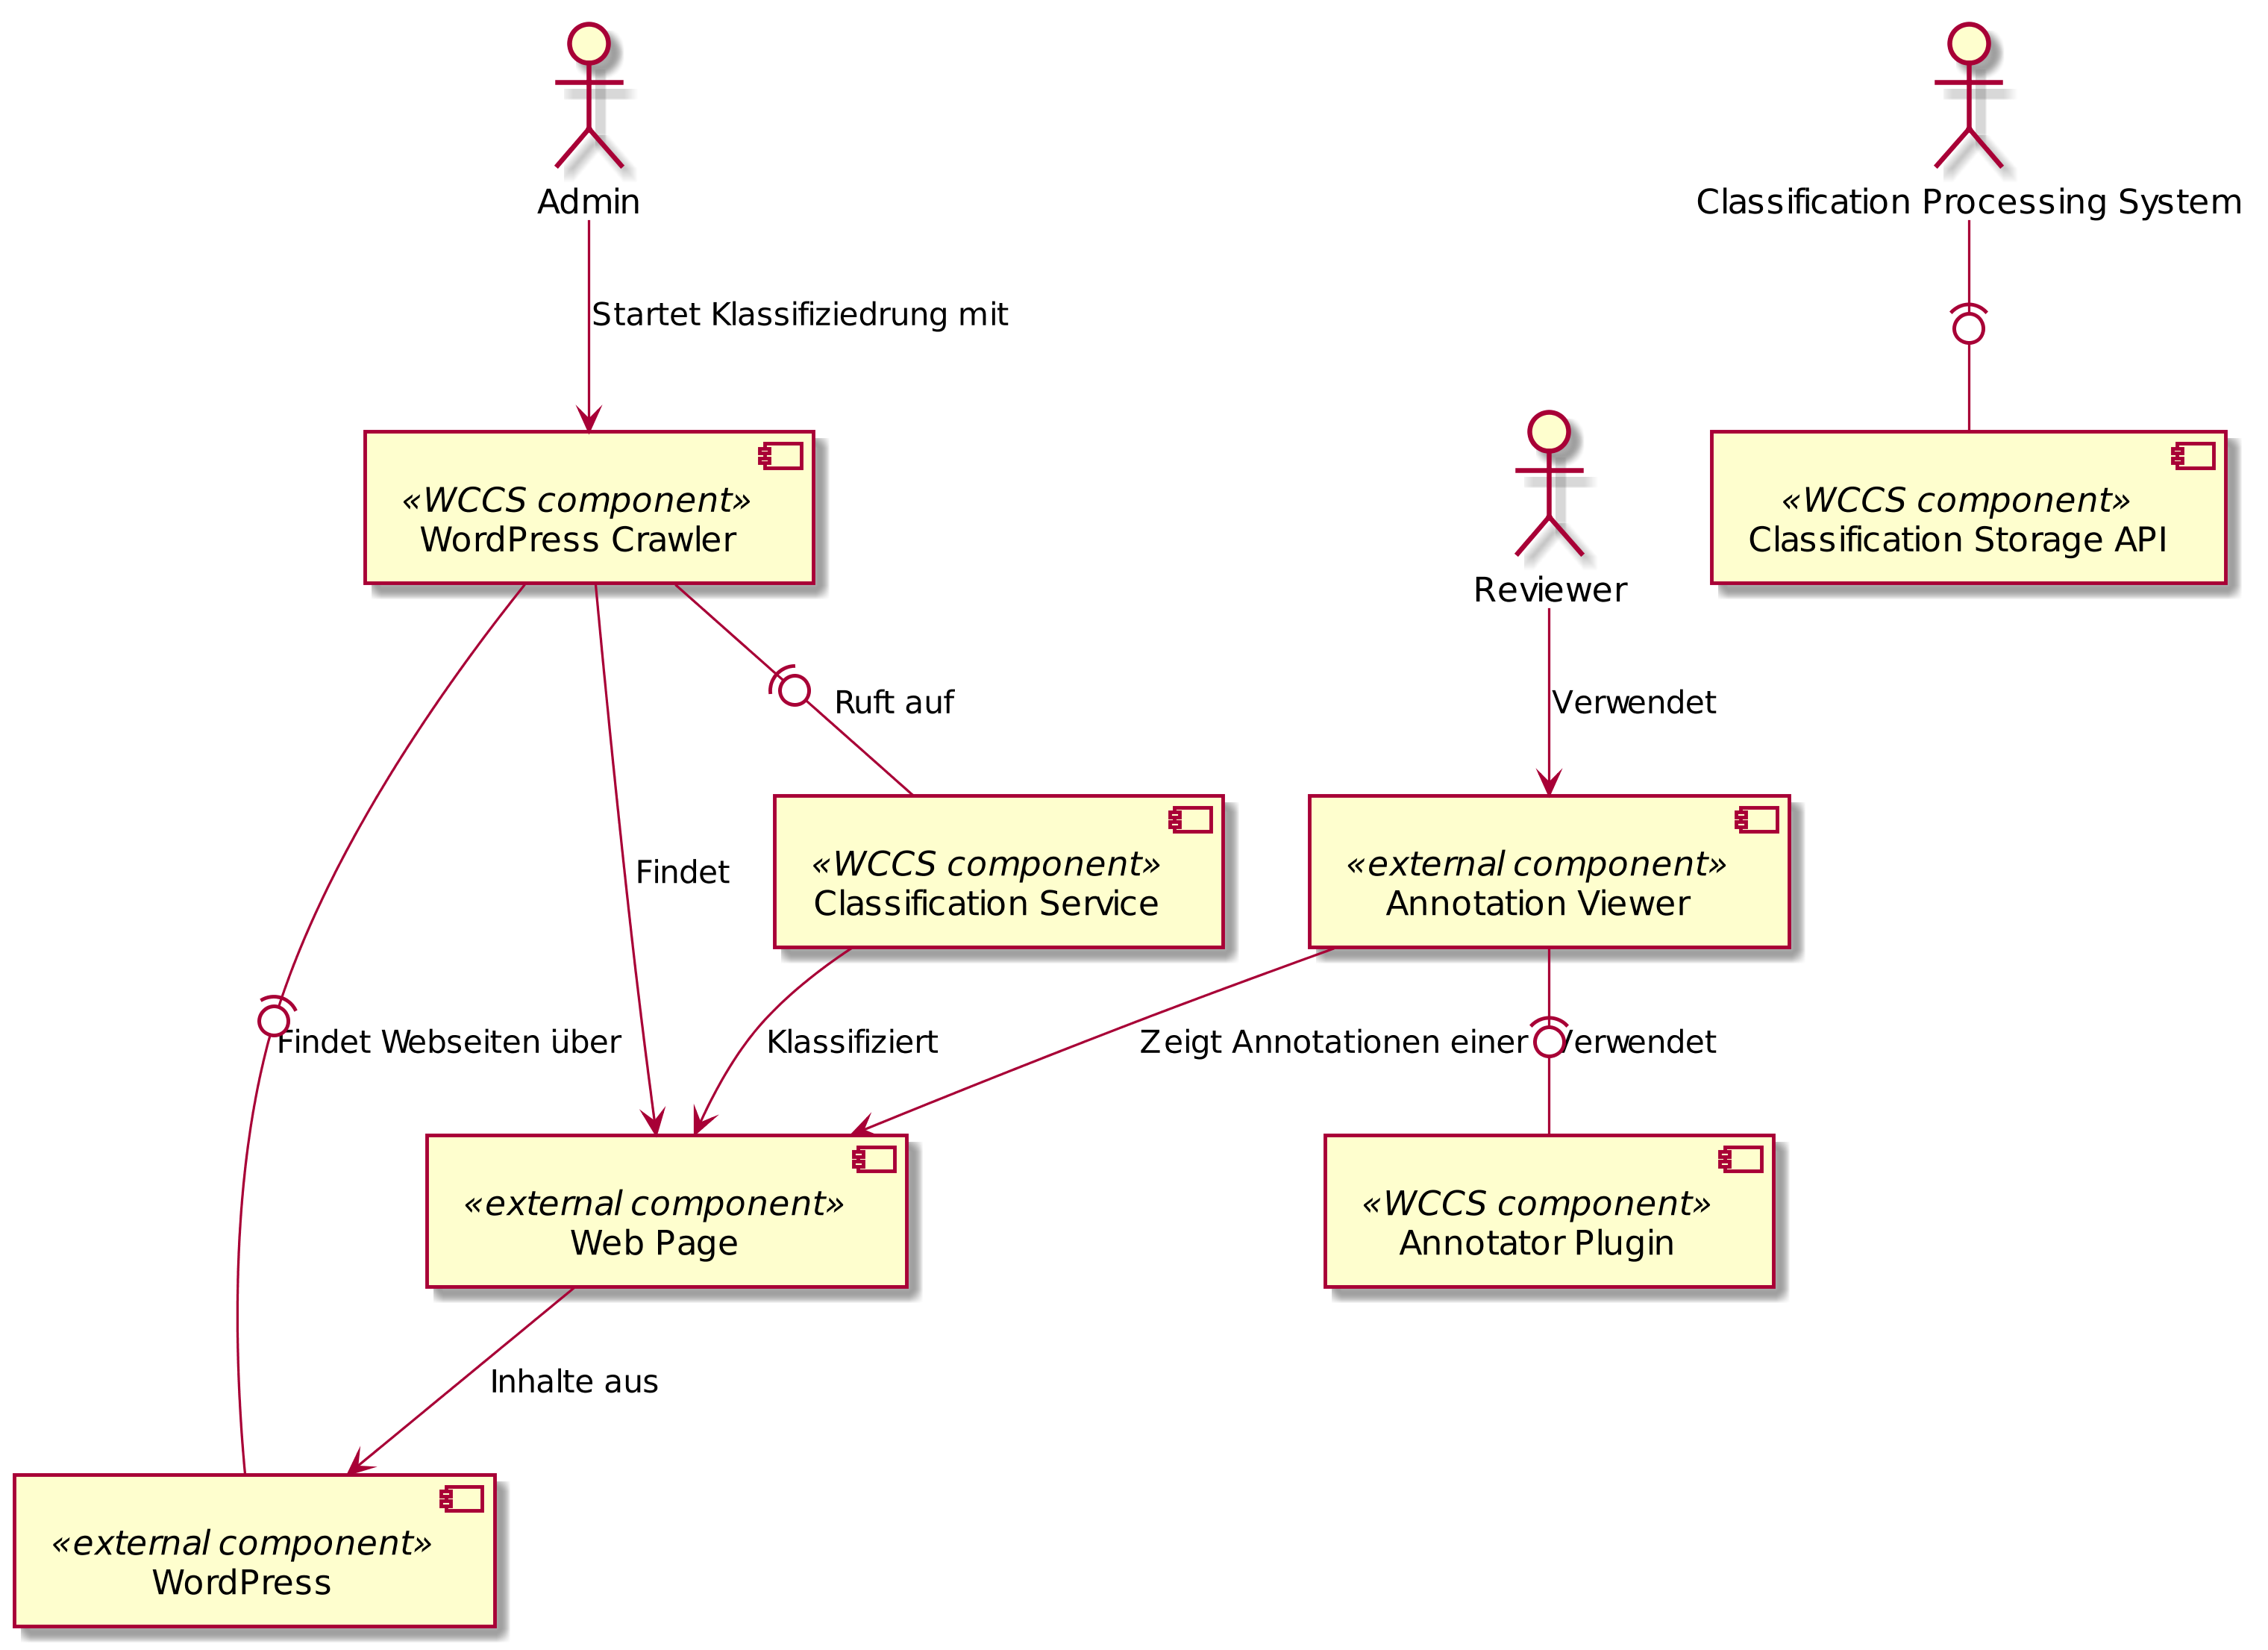
\includegraphics[width=\textwidth]{../resources/architecture/external_architecture.png}
            \caption{Externe Architkektur von WCCS}
            \label{image:wccsExternalArchitecture}
        \end{figure}

        Eine zentrale externe Komponente ist die Webseite,
        die Inhalte aus einem \gls{cms} - im konkreten Fall {\wordpress} -
        darstellt und vom Classification Service klassifiziert wird.
        Dazu startet der Admin den WordPress Crawler, der ebenfalls ein Teil des \gls{wccs} ist.
        Diese Komponente findet Webseiten über {\wordpress} und beauftragt den
        Classification Service diese zu klassifizieren.
        Obwohl Crawler Teil des \gls{wccs} ist, steht sie etwas außerhalb,
        da sie nur mit {\wordpress} funktioniert. Für andere Systeme muss ein anderes Tool
        entwickelt werden. Deshalb ist sie nicht so allgemeingültig.
        Konzeptionell gibt es aber immer so eine Komponente.
        Mehr in Kapitel \ref{section:solutionDetailsCrawler}.

        Nach der Klassifizierung kann eine externe Komponente das Annotator Plugin
        einbinden und damit die Annotationen visualisieren.
        Diese Komponente heißt deshalb Annotation Viewer und wird von einem Redakteur
        verwendet.

        Letzendlich können beliebige Drittsysteme die Classification Storage API
        nutzen, um Klassifikationen abzufragen und weiterzuverarbeiten.